\section{Mapserver Peta Singapore}
 +\subsection{Mapserver}
  Mapzen dibangun dari berbagai peralatan open-source yang dikemas ke dalam layanan Web dan di hosting di server Mapzen. Salah satu keunggulan Mapzen selain keterbukaannya adalah penggunaan mesin rendering fleksibel yang disebut Tangram untuk menampilkan peta digital dalam nuansa 2D maupun 3D secara real-time, sehingga membuat kartografi akan terlihat bagus dimana-saja.
  
 +\subsection{Cara Instalasi Mapserver}
 +\begin{enumerate}
 +\item
 +Download Mapserver atau disingkat MS4W di http://mapserver.org/download.html \ref{gambar1} seperti gambar dibawah ini
 +\begin{figure}[ht]
 +	    \centerline{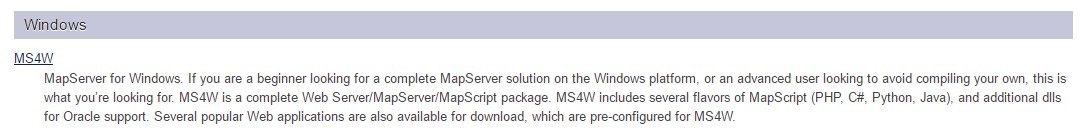
\includegraphics[width=0.50\textwidth]{figures/img1}}
 +	    \caption{Download MS4W}
 +		\label{gambar1}
 +		\end{figure}
 +\item
 +Setelah di download jalankan setupnya, disini saya menggunakan port 8080 karena port default 80 sudah dipakai oleh xampp \ref{gambar2} seperti gambar dibawah ini
 +\begin{figure}[ht]
 +	    \centerline{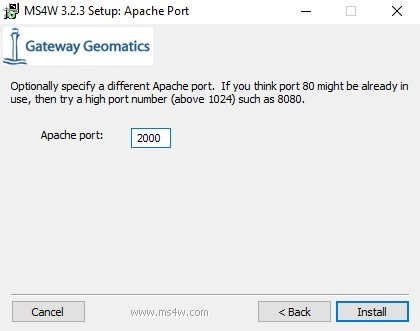
\includegraphics[width=0.50\textwidth]{figures/img2}}
 +	    \caption{Port 2000}
 +		\label{gambar2}
 +		\end{figure}
 +\item
 +Lalu tunggu instalasi sampai selesai \ref{gambar3} seperti gambar dibawah ini
 +\begin{figure}[ht]
 +	    \centerline{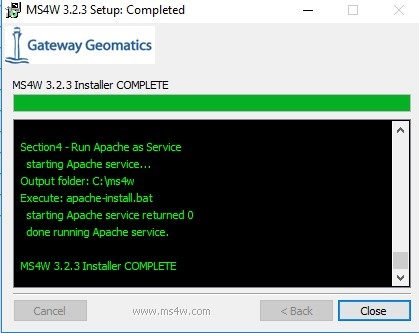
\includegraphics[width=0.50\textwidth]{figures/img3}}
 +	    \caption{Selesai}
 +		\label{gambar3}
 +		\end{figure}
 +\item
 +Setelah proses selesai silahkan buka browser favorit anda, kemudian ketikkan http://localhost:8080 di kotak isian URL.
 +\item
 +Jika anda melihat tampilan home MAPSERVER atau MS4W proses instalasi anda berhasil \ref{gambar4} seperti gambar dibawah ini
 +\begin{figure}[ht]
 +	    \centerline{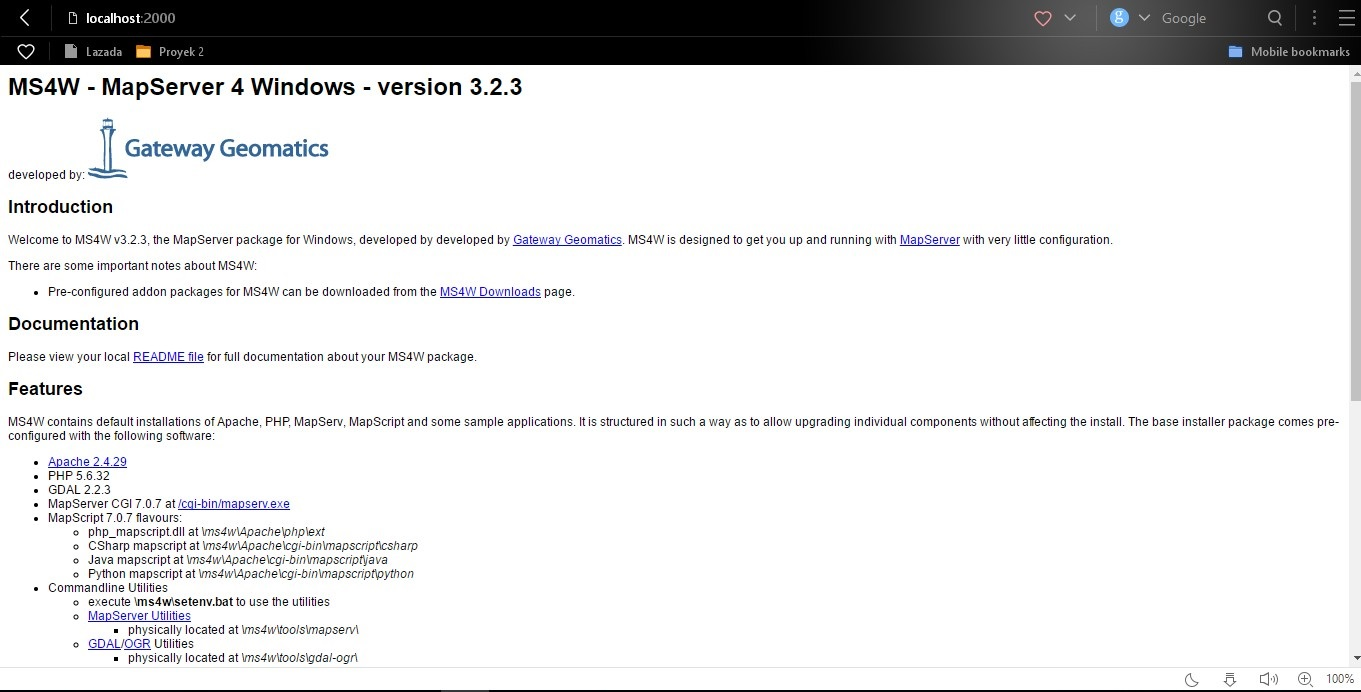
\includegraphics[width=0.50\textwidth]{figures/img4}}
 +	    \caption{Tampilan MS4W}
 +		\label{gambar4}
 +		\end{figure}
 +\end{enumerate}
 +Sekian Proses instalasi Mapserver pada Windows
 
 \subsection{File yang dibutuhkan di Mapserver}
File index.html simpan di folder C:\ms4w\Apache\htdocs\web. Untuk memanggil gambar peta melalui halaman html.
File peta.map simpan di folder C:\ms4w\apps\map. Untuk menyusun layer-layer peta (file *.shp).
File fdistrict.dbf,  fdistrict.sbn,  fdistrict.sbx,  fdistrict.shp,  fdistrict.shx simpan di folder C:\ms4w\apps\map\shp. Sebagai gambar digitalnya yang dibuat dengan aplikasi QuantumGIS.
File-file *.shp merupakan gambar digitalnya, gambarnya tersebut di hasilkan dengan bantuan aplikasi quantumGIS. Jadi gambar yang di tampilkan bukan gambar langsung dengan format *.jpg atau *.gif.
Adapun struktur folder pada aplikasi ms4w adalah seperti di bawah. Folder “web” berisi file-file web baik di buat dengan PHP atau HTML. Sedangkan folder “map” berisi file-file *.map yang berfungsi untuk mengatur tampilan peta digital, dan file-file di folder shp untuk gambar digitalnya.
\begin{figure}[ht]
 +	    \centerline{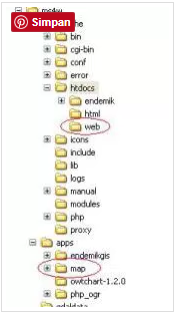
\includegraphics[width=0.50\textwidth]{figures/shp}}
 +	    \caption{file shp}
 +		\label{shp}
 +		\end{figure}
 +\end{enumerate}
 Selanjutnya untuk memanggil  aplikasi peta yang akan kita panggil kita harus membuat alias untuk memanggilnya dengan cara buka folder MS4w - httpd.d – httpd_nama. Disini untuk (http_nama ) saya menggunakan httpd_kabupaten lalu buka httpd_kabupaten dengan notepad++ lalu buat alias untuk pemanggilan pada browser. Setelah pembuatan alias telah beres selanjutnya kita coba panggil pada browser localhost/kabupaten/ dan hasilnya adalah sebagai berikut. Pertama untuk menampilkan peta indonesia beserta titik-titiknya terlebih dahulu kita harus memasukan 5 file yang telah dibuat sebelumnya di Quantum GIS yang menghasilkan file yang berextensi .shp dan lainnya. Lalu masukan kelima file tersebut kedalam folder MS4W – Apps – (nama_folder) Setelah kita masukan kelima file tersebut kedalam folder pmapper_demodata lalu kita buka MS4W – Apps – kabuapten – config – default – file.map, Disini untuk file.map saya memberi nama kabupaten.map lalu buka kabupaten.map tersebut dengan notepad++
 
 Fungsi dari referense adalah untuk mengetahui dimanakah posisi gambar ketika peta pada browser di Zoom in (diperbesar ) sehingga kita bisa mengetahui bahwa kita sedang melihat peta bagian mana. Disamping itu refernse juga bisa dipakai untuk menggeser secara langsung ketempat yang kita inginkan secara langsung tanpa harus kita mengecilkan gambar terlebih dahulu. Samakan extend referense dengan extend pada pengaturan peta indonesia diatas dan beri nama file gambar yang kita gunakan sesuai dengan nama gambar yang ada pada direktori penyimpanan yang disimpan pada folder Images.
 
 
